%
% This document is free; you can redistribute it and/or modify
% it under the terms of the GNU General Public License as published by
% the Free Software Foundation; either version 2 of the License, or
% (at your option) any later version.
%
% This document is distributed in the hope that it will be useful, but
% WITHOUT ANY WARRANTY; without even the implied warranty of
% MERCHANTABILITY or FITNESS FOR A PARTICULAR PURPOSE.  See the GNU
% General Public License for more details.
%
% You should have received a copy of the GNU General Public License
% along with this document; if not, write to the Free Software
% Foundation, Inc., 51 Franklin Street, Fifth Floor, Boston, MA
% 02110-1301, USA.
%
% Author: Bertoli Marco
%
\chapter{Introduction}
\emph{The Java Modelling Tools (JMT) is a free open source suite for
performance evaluation, capacity planning and modelling of computer
and communication systems. The suite implements numerous
state-of-the-art algorithms for the exact, asymptotic and simulative
analysis of queueing network models, either with or without
product-form solution. Models can be described either through wizard
dialogs or with a graphical user-friendly interface. The suite
includes also a workload analysis tool based on clustering
techniques. The suite incorporates an XML data layer that enables
full reusability of the computational engines.}

The JMT suite is composed of \emph{six} tools that support different
analyses frequently used in capacity planning studies. The main
features of each tool follows.

\medskip \noindent 
\includegraphics[scale=.5]{img/JSIMIcon}
\textbf{JSIM:} a discrete-event simulator for the analysis of queueing
network models. An intuitive sequence of \emph{wizard} windows helps
specifying network properties. The simulation engine supports
several probability distributions for characterizing service and
inter-arrival times. Load-dependent strategies using arbitrary
functions of the current queue-length can be specified. JSIM
supports state-independent routing strategies, e.g., Markovian or
round robin, as well as state-dependent strategies, e.g., routing to
the server with minimum utilization, or with the shortest response
time, or with minimum queue-length. The simulation engine supports
several extended features not allowed in product-form models,
namely, finite capacity regions (i.e., blocking), fork-join servers,
and priority classes. The analysis of simulation results employs
on-line transient detection techniques based on spectral analysis.
What-if analyses, where a sequence of simulations is run for
different values of parameters, are also possible.

\medskip \noindent 
\includegraphics[scale=.5]{img/JMODELIcon}
\textbf{JMODEL:} a graphical user-friendly interface for the simulator
engine used by JSIM. It integrates the same functionalities of JSIM
with an intuitive graphical workspace. This allows an easy
description of network structure, as well as a simplified definition
of the execution features like blocking regions. Network topologies
can be exported in vectorial or raster image formats.

\medskip \noindent 
\includegraphics[scale=.5]{img/JMVAIcon}
\textbf{JMVA:} meant for the exact analysis of single or multiclass
product-form queueing network models, either processing open, closed
or mixed workloads. The classic MVA solution algorithm is used.
Network structure is specified by textual \emph{wizards}, with
conversion functions from probabilities to average visit ratios (and
viceversa). What-if analyses are allowed.

\medskip \noindent 
\includegraphics[scale=.5]{img/JMCHIcon}
\textbf{JMCH:} it applies a simulation technique to solve a single
station model, with finite (M/M/1/k) or infinite queue (M/M/1), and
shows the underlying Markov Chain. It is also possible to
dynamically change the arrival rate and service time of the system.

\medskip \noindent 
\includegraphics[scale=.5]{img/JABAIcon}
\textbf{JABA:} a tool for the identification of bottlenecks in closed
product-form networks using efficient convex hull algorithms. The
tool supports models with up to three job classes. It is possible to
identify potential bottlenecks corresponding to the different mixes
of customer classes. Models with thousands of queues can be analyzed
efficiently. The saturation sectors, i.e., the mixes of customer
classes that saturate more than one resource simultaneously, are
identified.

\medskip \noindent 
\includegraphics[scale=.5]{img/JWATIcon}
\textbf{JWAT:} supports the workload characterization phase, with
emphasis on Web log data. Some standard formats for input file are
provided (e.g., Apache HTTP log files), and customized formats may
also be specified. The imported data can initially be analyzed using
descriptive statistical techniques (e.g, means, correlations, pdf
histograms, boxplots, scatterplots), either for univariate or
multivariate data. Algorithms for data scaling, sample extraction,
outlier filtering, k-means and fuzzy k-means clustering for
identifying similarities in the input data are provided. These
techniques allow to determine cluster centroids, and then estimate
mean workload and service demands to be used for model
parametrization. The tool includes also an interface to the
similarity clustering tool CLUTO.

\section{Starting the JMT suite}
Double click on the JMT icon

\includegraphics[scale=.5]{img/JMTIcon} on your \emph{program group} or
\emph{desktop}, or open the \emph{command prompt} and type from the
installation directory:
\begin{verbatim}
    java -jar JMT.jar
\end{verbatim}
the window of \autoref{fig:startscreen} will be shown.

\begin{figure}[htbp]
    \begin{center}
        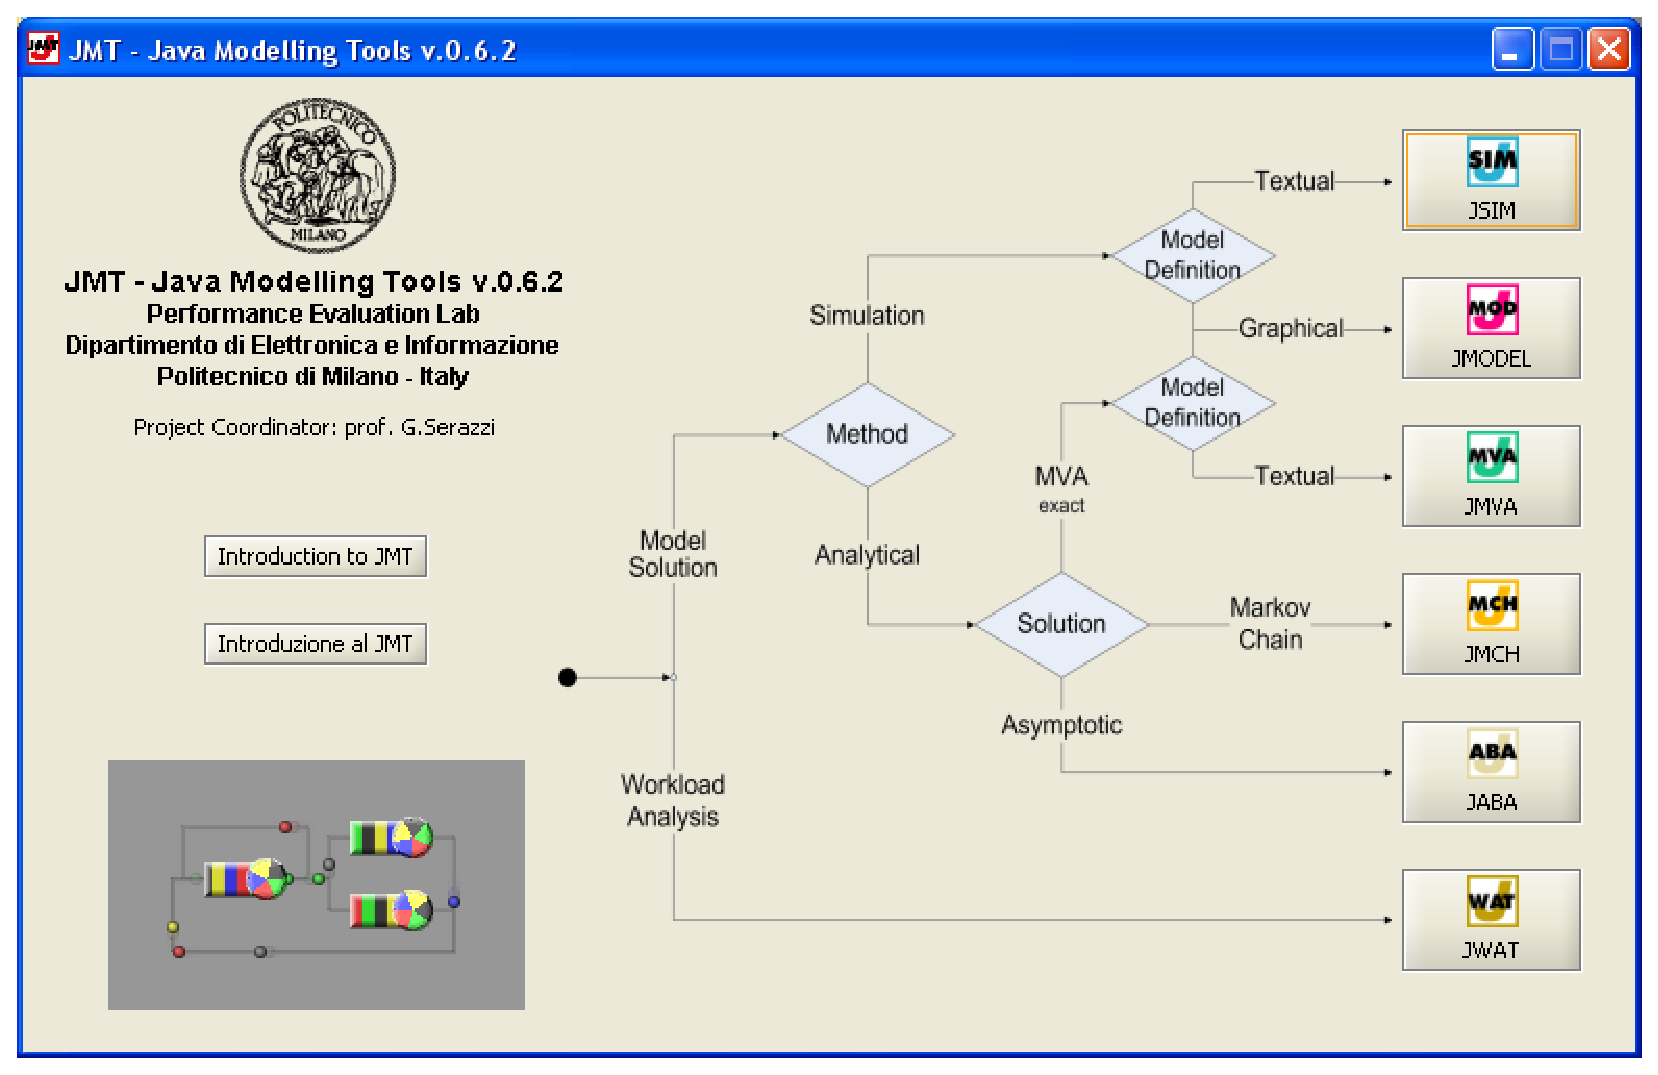
\includegraphics[scale=.5]{img/StartScreen}
    \end{center}
    \caption{JMT suite Starting Screen}
    \label{fig:startscreen}
\end{figure}

This starting screen is used to select the application of the suite
to be executed by clicking on the corresponding button. The flow
chart try to help the user to chose the application that best fits
its needs.

In the following chapters all of the tools\footnote{for the moment
only \emph{JMVA}} will be examined with details and examples. This
manual is intended for the general user that wants to learn how to
interact with Java Modelling Tools; advanced users that want to
learn details on internal data structures, computational engines and
XML interfaces should refer to \emph{JMT system manual}.
